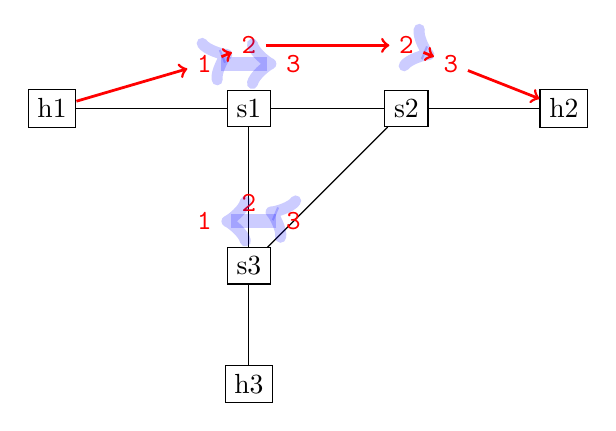
\begin{tikzpicture}[node distance=0.8cm]
\tikzstyle{host}=[draw]
\tikzstyle{switch}=[draw]
\tikzstyle{connection}=[]
\tikzstyle{constr}=[above,sloped,font=\ttfamily\small]
\tikzstyle{moreconstr} = [constr,below]
\tikzstyle{port}=[red,font=\ttfamily]
\tikzstyle{passing}=[->,bend left, line width=1pt,red]
\tikzstyle{send}=[->,line width=5pt,blue,opacity=0.2]
\node[host] (h1) at (-0.5,-0.5) {h1};
\node[host] (h2) at (6,-0.5) {h2};
\node[host] (h3) at (2,-4) {h3};
\node [switch] (s1) at (2,-0.5) {s1};
\node [switch] (s2) at (4,-0.5) {s2};
\node [switch] (s3) at (2,-2.5) {s3};
\draw [connection] (h1) edge (s1);
\draw [connection] (s1) edge (s2);
\draw [connection] (s2) edge (h2);
\draw [connection] (s1) edge (s3);
\draw [connection] (s3) edge (h3);
\draw [connection] (s2) edge (s3);
\node [above left of=s1,port] (s1p1) {1};
\node [above of=s1,port] (s1p2) {2};
\node [above right of=s1,port] (s1p3) {3};
\node [above of=s2,port] (s2p2) {2};
\node [above right of=s2,port] (s2p3) {3};
\node [above left of=s3,port] (s3p1) {1};
\node [above of=s3,port] (s3p2) {2};
\node [above right of=s3,port] (s3p3) {3};

\draw[send] (s1p1) -- (s1p2);
\draw[send] (s1p1) -- (s1p3);
\draw[send] (s2p2) -- (s2p3);
\draw[send] (s3p3) -- (s3p1);
\draw[send] (s3p3) -- (s3p2);

\draw[passing] (h1) -- (s1p1);
\draw[passing] (s1p1) -- (s1p2);
\draw[passing] (s1p2) -- (s2p2);
\draw[passing] (s2p2) -- (s2p3);
\draw[passing] (s2p3) -- (h2);

\end{tikzpicture}